\newpage
\section{Cosa è l'analisi delle immagini satellitari}
L'analisi delle immagini satellitari si riferisce al processo di estrazione di informazioni importanti dalle fotografie aeree scattate da satelliti orbitali.
Questo campo combina la disciplina del telerilevamento con tecniche di apprendimento automatico (nello specifico computer vision) per interpretare grandi quantità di dati visivi.
\subsection{Dati di una fotografia satellitare}
All'interno di una fotografia comune (banalmente anche quella scattata dai telefoni), è possibile ricavarne i colori attraverso la codifica RGB che sta per Red (Rosso), 
Green (Verde) e Blue (Blu). Attraverso la combinazione di questi 3 valori si possono ricreare tutti i colori dello spettro 
visibile (osservabile con gli occhi). Inoltre, nelle immagini satellitari, vi sono anche i canali infrarosso quali 
RedEdge, NIR e SWIR.
Si mostra una tabella \ref{tab:tabella infrarosso} di alcune frequenze d'onda della radiazione 
elettromagnetica. A ogni frequenza appartiene una categoria. Si mostra anche un'immagine \ref{fig:spettro infrarosso} che illustra lo spettro della luce visibile e dell'infrarosso.
\begin{table}[htbp]
    
    \begin{center}
    \begin{tabular}{|c|c|}
    \hline
    Tipologia & Lunghezza d'onda \\
    \hline
    Viola & $\sim 380-450 nm$ \\
    Blu & $\sim 450-495 nm$ \\
    Verde & $\sim 495-570 nm$ \\ 
    Giallo & $\sim 570-590 nm$ \\
    Arancione & $\sim 590-620 nm$ \\
    Rosso & $\sim 620-705 nm$ \\
    RedEdge & $\sim 705-740 nm$ \\
    NIR & $\sim 760-900 nm$ \\
    SWIR & $\sim 1150-2350 nm$ \\

    \hline
    \end{tabular}
    \caption{tabella infrarosso}
    \label{tab:tabella infrarosso}
    \end{center}
\end{table}

\begin{figure}[htbp]
    \centering
    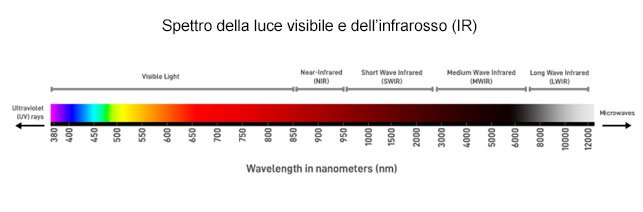
\includegraphics[width=0.7\textwidth]{capitoli/capitolo1/images/Spettro-luce-visibile-e-infrarosso.png}
    \caption{spettro della radiazione visibile e dell'infrarosso}
    \label{fig:spettro infrarosso}
\end{figure}
Attraverso l'infrarosso si può comprendere caratteristiche invisibili all'occhio umano per esempio lo stato di salute della vegetazione o i livelli di umidità del suolo.
\\Per lavorare con questi tipi di immagini è stato usato il software open source QGIS. Queste immagini hanno un formato \texttt{.tiff} e i file con cui è stato lavorato sono chiamati \texttt{...6band.tiff} dove, in questo caso, \texttt{6band} sta per $Red+Green+Blue+RedEdge+NIR+SWIR$.
I valori delle bande nei file \texttt{.tiff} satellitari vengono salvati come \texttt{float32}. Questo formato permette di rappresentare le variabili con la virgola mobile. Questo viene fatto per avere una precisione maggiore, anziché l'utilizzo di numeri interi.\\
Un esempio di un'immagine satellitare, con bbox (bounding box) disegnate per indicare la pianta, è riportata \ref{fig:satellite con identificazione piante}.
Le bbox vengono salvate in file \texttt{.geojson}. All'interno di questo file ogni riga appartiene a una singola bbox e ogni riga contiene le coordinate dei punti che formano il poligono (cioè la bbox).
\begin{figure}[htbp]
    \centering
    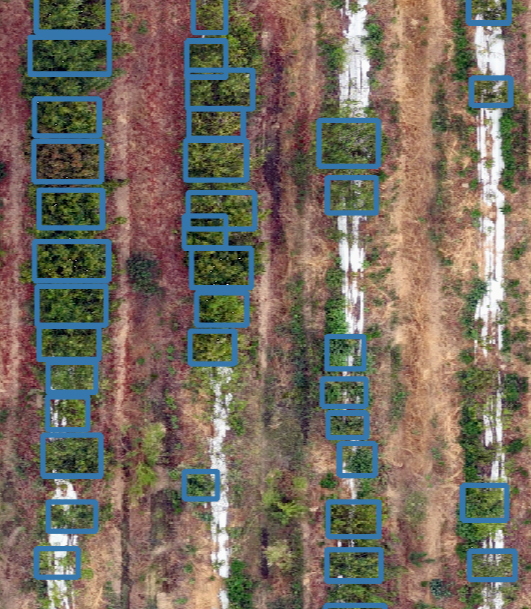
\includegraphics[width=0.7\textwidth]{capitoli/capitolo1/images/satellite.png}
    \caption{Immagine satellitare con identificazione piante}
    \label{fig:satellite con identificazione piante}
\end{figure}
\\Un'immagine è un insieme di pixel con coordinate $(x,y)$ dove $x$ mi indica la posizione del pixel nell'immagine sull'asse delle ascisse (asse orizzontale) e $y$ sull'asse delle ordinate (asse verticale).
Ogni pixel, oltre alle coordinate di riferimento, ha un valore che indica l'intensità del rosso, uno del verde, uno del blu, uno del RedEdge, uno del NIR e uno del canale SWIR.
\section{Introduzione al Machine Learning}
Il machine learning è il sottoinsieme dell'intelligenza artificiale (AI) basato su algoritmi in grado di "apprendere" i modelli dei dati di addestramento e, successivamente, fare previsioni accurate sui nuovi dati. 
Questa capacità di riconoscimento dei modelli consente ai modelli di machine learning di prendere decisioni o fare previsioni senza istruzioni esplicite e codificate.\\
Si definisce \texttt{dati di addestramento} o \texttt{training data} una parte di dati di un dataset che verrà usata per allenare il modello. Il dataset
viene definito come un insieme di dati organizzati $(X = x_1,..., x_n)$, dove a ogni elemento facente parte di esso, detto istanza o sample, rappresenta una misurazione
di un certo fenomeno di interesse.\\
Un esempio di un dataset potrebbe essere quello di una farmacia \ref{tab:dataset_farmacia}.
\begin{table}[h]
\centering
\begin{tabular}{|c|l|l|c|c|}
\hline
\textbf{Esempio} & Farmaco & Categoria & Prezzo & Disponibilità \\
\hline
$x_1$ & Tachipirina 1000 mg & Analgesico & 7.50 & Disponibile \\
$x_2$ & Aspirina 500 mg & Antinfiammatorio & 5.20 & Disponibile \\
$x_3$ & Moment 200 mg & Antidolorifico & 6.80 & Esaurito \\
$x_4$ & Augmentin 875 mg & Antibiotico & 12.40 & Disponibile \\
$x_5$ & Enterogermina & Probiotico & 9.90 & Disponibile \\
$x_6$ & Benagol Gola & Pastiglie gola & 4.30 & Disponibile \\
$x_7$ & Voltaren Gel & Antinfiammatorio & 10.50 & Esaurito \\
$x_8$ & Zyrtec 10 mg & Antistaminico & 8.70 & Disponibile \\
\hline
\end{tabular}
\caption{Esempio di dataset relativo ai prodotti di una farmacia}
\label{tab:dataset_farmacia}
\end{table}

\subsection{Tipologie di apprendimento}
Possiamo distinguere i modelli di machine learning in 3 principali tipi di apprendimento automatico:
\begin{itemize}
    \item \textbf{Apprendimento Supervisionato}:\\
    Nel dataset all'input $x_i$ viene associato (a ogni input $x_i$) un output $y_i$. Si riporta una tabella esempio \ref{tab:coppie_dataset_farmacia}. 
    In questo caso $y_i$ indica se deve essere comprato oppure no il farmaco dal grossista.
    \begin{table}[H]
    \centering
    \begin{tabular}{|c|l|l|c|c|}
    \hline
    \textbf{Input} & \textbf{Output}:Comprare?\\
    \hline
    $x_1$ & $y_1=SI$ \\
    $x_2$ & $y_2=NO$ \\
    $x_3$ & $y_3=NO$ \\
    $x_4$ & $y_4=SI$ \\
    $x_5$ & $Y_5=SI$ \\
    $x_6$ & $y_6=NO$ \\
    $x_7$ & $y_7=SI$ \\
    $x_8$ & $y_8=SI$ \\
    \hline
    \end{tabular}
    \caption{Esempio di coppie di un dataset}
    \label{tab:coppie_dataset_farmacia}
    \end{table}
    Il modello osserva coppie di input-output ($(x_1,y_1),...,(x_n,y_n)$) e apprende una funzione (chiamata $\hat{h}$) che dato l'input ($x_i$), il valore della funzione $\hat{h}(x_i)$ cerca di farlo avvicinare all'output corretto ($y_i$). Per esempio, gli input potrebbero essere
    immagini ottenute da una fotocamera, ognuna accompagnata da un output che indica “bus”
    o “pedone” e così via. Un output come questo è chiamato etichetta. Nel nostro esempio l'output è se il farmacista dovrebbe comprare il medicinale dal grossista oppure no, mentre le etichette sono Farmaco, Categoria, Prezzo e Disponibilità.
    Una funzione è dato un input $x_i$ si ricava il risultato. Per esempio la funzione
    \begin{align}
        h(x_i)&=y_i\\
        h(x_i)&=2x_i+3\\
        h(3)&=2\cdot 3+3=9
    \end{align}
    Tuttavia, nel machine learning, la forma della funzione ($2x+3$) non viene fissata in anticipo: non la conosciamo. 
    Questa è calcolata automaticamente a partire dai dati di addestramento.
    \item \textbf{Apprendimento Non Supervisionato}:\\
    Il modello apprende i pattern dall'input ($x_i$) senza alcun
    feedback esplicito ($y_i$). L'attività di apprendimento non supervisionato più comune è il clustering: 
    individuare cluster potenzialmente utili di esempi di input. Per esempio, un sistema
    di visione artificiale, osservando milioni di immagini prese da Internet, è in grado di
    identificare un ampio cluster di immagini simili che una persona chiamerebbe gatti.
    Per esempio nell'immagine sottostante \ref{fig:cluster} i puntini in rosso sono i gatti, in verde le piante e in blu i pesci. 
    \begin{figure}[htbp]
        \centering
        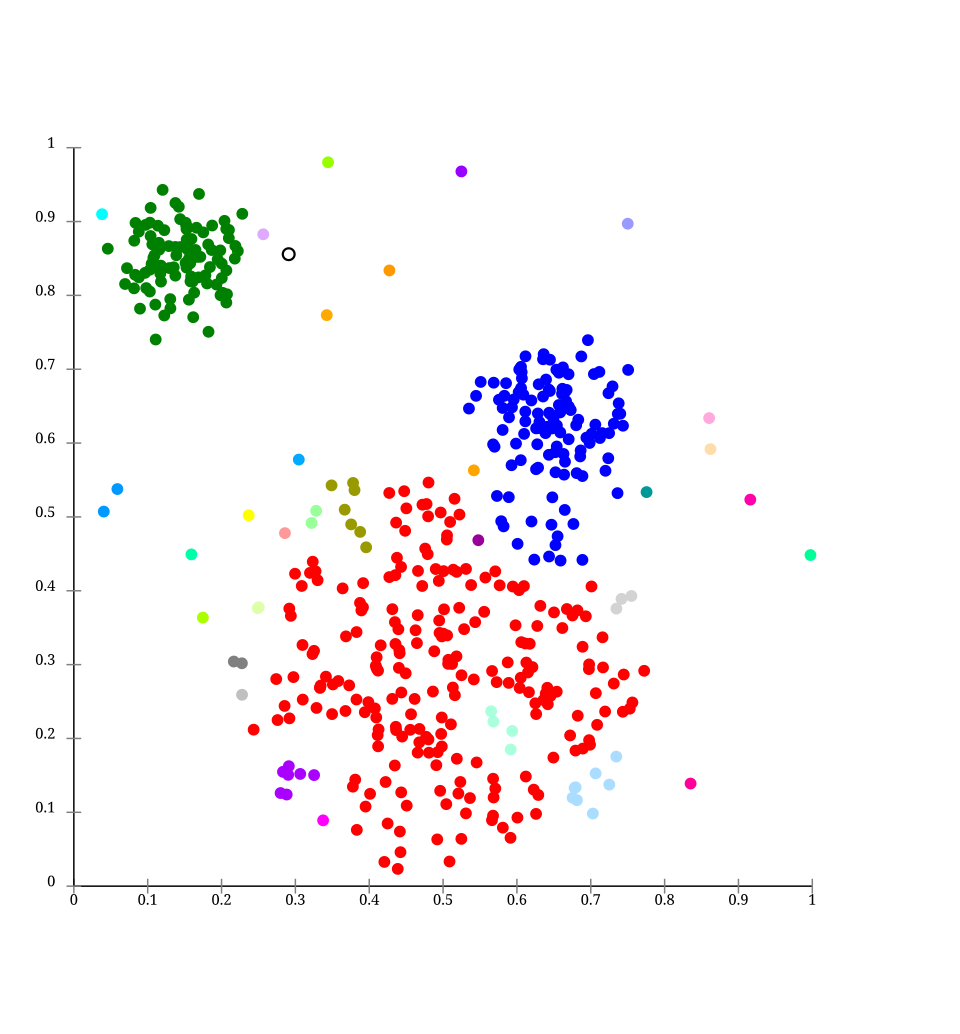
\includegraphics[width=0.5\textwidth]{capitoli/capitolo1/images/SLINK-Gaussian-data.png}
        \caption{Rappresentazione di un cluster di un dataset}
        \label{fig:cluster}
    \end{figure}
    \item \textbf{Apprendimento Rinforzato}:\\
    L'apprendimento avviene grazie a una serie di rinforzi: il modello impara da risposte positive o negative sul risultato. Ad esempio, dopo una partita a
    un gioco scelto, possono essere assegnati premi per la vittoria o punizioni per la sconfitta in base
    a come ha giocato il modello. Il gioco viene ripetuto e le azioni e scelte prese vengono
    progressivamente alterate dal modello in modo che questo ricerchi una ricompensa.
\end{itemize}

In questa tesi si andrà a lavorare con la tipologia di apprendimento supervisionato.

\subsection{Apprendimento Simbolico e Non Simbolico}
Il machine learning simbolico è un approccio all'apprendimento automatico che si basa sulla rappresentazione esplicita della conoscenza, tramite simboli (cioè segni che indicano entità, categorie e relazioni che vogliamo rappresentare 
(ad esempio \texttt{gatto}, \texttt{essere vivente}, \texttt{appartiene a})), regole logiche espresse tipicamente come implicazioni (se succede questo, allora...) e inferenza (ragionamento deduttivo).\\
Un esempio di ragionamento deduttivo è il seguente:
a partire da regole generali e da fatti specifici, una macchina deduce 
una conclusione logicamente necessaria (se è vero che \texttt{tutti i mammiferi allattano} 
e che \texttt{Fido è un mammifero}, allora deduco che \texttt{Fido allatta}).\\
L'apprendimento simbolico non necessita di grandi quantità di dati per l'addestramento, ha un'alta trasparenza nelle decisioni (perché ogni ragionamento si può comprendere attraverso regole logiche) e ha limiti nella gestione di dati rumorosi o ambigui.\\
L'apprendimento simbolico si contrappone all'apprendimento statistico (ad esempio le reti neurali), 
basato su correlazioni numeriche estratte dai dati. Quest'ultimo ha bisogno di grandi quantità di dati nell'apprendimento, sono delle blackbox (dato un input si ha un output, ma non si conosce il ragionamento dietro) e è buono nella gestione di dati rumorosi o ambigui.

\subsection{Bontà del modello}
Per valutare se il modello è buono per il problema si necessità di conoscere i seguenti parametri.
\begin{itemize}
    \item F1-macro     
    \item ROC-AUC    
    \item Prec-macro    
    \item Rec-macro
\end{itemize}
\begin{itemize}
    \item Positivi Veri ($PV_i$): pixel correttamente predetti come positivi;
    \item Negativi Veri ($NV_i$): pixel correttamente predetti come negativi;
    \item Positivi Falsi ($PF_i$) - pixel negativi ma predetti positivi;
    \item Negativi Falsi ($NF_i$) - pixel positivi ma predetti negativi.
\end{itemize}

Da qui si riesce a calcolare le seguenti formule:

\begin{itemize}
    \item $Precision_i$: proporzione dei pixel classificati come piante e che rappresentano
effettivamente delle piante.
\[
Precision_i=\frac{PV_i}{PV_i+PF_i}
\]
    \item $Recall_i$: calcola la percentuale di obiettivi da riconoscere che sono stati
riconosciuti.
\[
Recall_i=\frac{PV_i}{PV_i + NF_i}
\]
    \item $F1_i$:serve per valutare la qualità di un modello
    \[
    F1_i=2\cdot\frac{Precision_i\cdot Recall_i}{Precision_i+Recall_i}
    \]
\end{itemize}
\begin{align}
    \text{Prec-macro}&=\frac{1}{N}\sum^N_{i=1}Precision_i\\
    \text{Rec-macro}&=\frac{1}{N}\sum^N_{i=1}Recall_i\\
    \text{F1-macro}&=\frac{1}{N}\sum^N_{i=1}F1_i
\end{align}

\subsection{Alberi Decisionali}
Possiamo visualizzare la tabella \ref{tab:dataset_farmacia} e \ref{tab:coppie_dataset_farmacia} come un albero decisionale \ref{fig:albero_farmacia}.
\begin{figure}[htbp]
\centering

\begin{tikzpicture}[scale=0.8]
% Stile nodi
\tikzstyle{decision} = [
    rectangle,
    draw,
    aspect=1,
    align=center
]

\tikzstyle{leaf} = [
    rectangle,
    rounded corners,
    draw,
    align=center
]

% Nodi
\node[decision] (root) at (0,0)
{Categoria};

\node[decision] (d1) at (-6,-3)
{Disponibile?};

\node[decision] (d2) at (6,-3)
{Prezzo};

\node[leaf] (n1) at (-6,-6)
{$y = NO$};

\node[leaf] (n6) at (-1.5,-3)
{$y = SI$};

\node[leaf] (n7) at (2,-3)
{$y = SI$};

\node[leaf] (n2) at (-3,-6)
{$y = SI$};

\node[leaf] (n3) at (2,-6)
{$y = SI$};

\node[decision] (d3) at (6,-6)
{Disponibile?};

\node[leaf] (n4) at (4,-9)
{$y = NO$};

\node[leaf] (n5) at (8,-9)
{$y = SI$};

% Archi
\draw[->] (root) -- node[left] {Antinfiammatorio} (d1);

\draw[->] (root) -- node[right] {...} (d2);

\draw[->] (root) -- node[right] {Prob} (n6);

\draw[->] (root) -- node[right] {Antibi} (n7);

\draw[->] (d1) -- node[left] {NO} (n1);

\draw[->] (d1) -- node[right] {SI} (n2);

\draw[->] (d2) -- node[left] {$\leq7$} (n3);

\draw[->] (d2) -- node[right] {$>7$} (d3);

\draw[->] (d3) -- node[left] {NO} (n4);

\draw[->] (d3) -- node[right] {SI} (n5);

\end{tikzpicture}

\caption{Albero decisionale del dataset farmacia}
\label{fig:albero_farmacia}

\end{figure}
\\Un albero decisionale serve a risolvere problemi di regressione e di classificazione \ref{fig:cluster}. Questo è una rappresentazione di una funzione
che dato in input un vettore di valori $x_i$ da un valore di output (una decisione) $y_i$ 
Ogni nodo interno all'albero corrisponde a un attributo della tabella, mentre i nodi esterni (foglie) a delle decisioni ($y=SI$ $y=NO$). 
I rami etichettati con degli ipotetici valori dell'attributo (Es. \texttt{Antinfiammatorio}, \texttt{SI}, \texttt{NO},...). Per \texttt{...} si intendono tutti gli altri 
elementi che non fanno parte di quella categoria e le diciture \texttt{Prob} e \texttt{Antibi} stanno per rispettivamente 
Probiotico e Antibiotico. Questo albero in particolare come si può osservare viene usato per una classificazione binaria ($y=0$ o $y=1$)($y=SI$ $y=NO$), ma si possono anche avere più classi ($y=0$, $y=1$, $y=2$) 
\subsection{Entropia}
\label{subsec:entropia}
Si può costruire un gran numero di alberi semplicemente cambiando attributi dell'albero. Per scegliere gli attributi e l'ordine di questi con cui costruire l'albero si usa il concetto
di guadagno di informazione \ref{subsec:guadagno_informativo}, definito in termini di entropia. L'entropia è la misura dell'incertezza di una variabile casuale.\\
L'unita di misura dell'entropia in questo caso (dato che si sta usando un computer (che comunica attraverso 0 o 1)) è il bit.

\subsubsection{Entropia di una singola variabile casuale}
L'entropia di una variabile casuale discreta $V$ con $k$ elementi è definita come:
\[
H(V)=-\sum_k P(v_k)\log_2P(v_k)
\]
Dove $v_k$ sono i possibili valori che la variabile aleatoria $V$ assume.
Ognuno di questi valori ha una probabilità $P(v_k) \in [0,1]$ di accadere. Inoltre $\sum_k P(v_k)=1$.
Per esempio il lancio di una moneta $4$ volte. La moneta ha $2$ possibilità eque (Testa o Croce). 
Quindi $V$ sarà un vettore lungo $k=16$ che contiene tutte i possibili lanci:
\begin{align}
    V&=
        \{TTTT,TTTC,TTCT,...,CCCC\}\\
    P(v_k)&=\left( \frac{1}{2} \right)^4\\
    P(V)&=
    \left\{
        \left( \frac{1}{2} \right)^4,
        \left( \frac{1}{2} \right)^4,
        \dots,
        \left( \frac{1}{2} \right)^4
    \right\}
\end{align}
Ad esempio
\begin{align}
    P(v_k=TCTT)&=\frac{1}{2}\cdot\frac{1}{2}\cdot\frac{1}{2}\cdot\frac{1}{2}= \frac{1}{16}\\
    H(V)&=-\sum_{k=1}^{k=16} \frac{1}{16}\log_2 \frac{1}{16}= 4\text{bit}
\end{align}
Quindi per rappresentare un risultato o i risultati dei $k$ elementi della variabile aleatoria $V$ sono necessari 4 bit.
La probabilità di ottenere C o T è $\frac{1}{2}$ e da qui si può affermare che la probabilità di ottenere un qualsiasi lancio di moneta 4 volte ($P(v_k)$) è esattamente $\left(\frac{1}{2}\right)^4$.\\


Ora, per esempio, si pone di avere una moneta truccata che dia T il $\frac{2}{3}$ dei lanci e C il restante $\frac{1}{3}$.
Di conseguenza
\begin{align}
    P(v_k=TCTT)&=\frac{2}{3}\cdot\frac{1}{3}\cdot\frac{2}{3}\cdot\frac{1}{3}= \frac{8}{81}\\
    P(v_k=TCCT)&=\frac{2}{3}\cdot\frac{1}{3}\cdot\frac{2}{3}\cdot\frac{1}{3}= \frac{4}{81}\\
    P(v_k=TCCC)&=\frac{2}{3}\cdot\frac{1}{3}\cdot\frac{2}{3}\cdot\frac{1}{3}= \frac{2}{81}\\
    P(v_k=TTTT)&=\frac{2}{3}\cdot\frac{1}{3}\cdot\frac{2}{3}\cdot\frac{1}{3}= \frac{16}{81}\\
    P(v_k=CCCC)&=\frac{2}{3}\cdot\frac{1}{3}\cdot\frac{2}{3}\cdot\frac{1}{3}= \frac{1}{81}
\end{align}
Per la sequenza TCTT, che contiene una sola C, si ottengono in totale 4 configurazioni distinte 
(ad esempio TCTT,CTTT,TTCT,TTTC). Analogamente, le sequenze con 2 C sono 4, quelle con 3 C sono anch'esse 4, 
mentre esistono un'unica configurazione con 4 C (CCCC) e una con 0 C (TTTT).
Quindi
\begin{align*}
    H(V)&=-\sum_k P(v_k)\log_2P(v_k)\\
    &=-\Bigg(\left(\frac{8}{81}\log_2\frac{8}{81}\right)\cdot4\\
    &\quad +\left(\frac{4}{81}\log_2\frac{4}{81}\right)\cdot4\\
    &\quad +\left(\frac{2}{81}\log_2\frac{2}{81}\right)\cdot4\\
    &\quad +\frac{16}{81}\log_2\frac{16}{81}+\frac{1}{81}\log_2\frac{1}{81}\Bigg)=3.2446
\end{align*}
Di conseguenza ci servono meno bit di informazione per rappresentare questo caso rispetto il precedente
\subsubsection{Entropia Congiunta}
Prese 2 variabili aleatorie discrete $V$ e $G$, l'entropia della loro coppia $(V,G)$ è:
%Poniamo qui un grafico di 2 insiemi
\[
H(V,G)=-\sum_{v,g}P(v_k,g_k)\log_2P(v_k,g_k)
\]
\usetikzlibrary{shapes,backgrounds}
\def\firstcircle{(0,0) circle (2.5cm)}
\def\secondcircle{(2,0) circle (2.5cm)}
\def\thirdcircle{(1,0)}
\begin{figure}[htbp]
    \begin{tikzpicture}
        \begin{scope}[ fill opacity=0.5]
            \fill[red] \firstcircle;
            \fill[green] \secondcircle;
            \draw \firstcircle node at (-1.5,0) {$H(V|G)$};
            \draw \secondcircle node at (3.5,0) {$H(G|V)$};
            \draw \thirdcircle node at (1.0,0) {$I(V,G)$};        
        \end{scope}
        % Legenda
        \draw[fill=red, opacity=0.5] (6,1) rectangle (6.5,1.5);
        \node[right] at (6.5,1.25) {Entropie individuali $H(V)$};

        \draw[fill=green, opacity=0.5] (6,0) rectangle (6.5,0.5);
        \node[right] at (6.5,0.25) {Entropie individuali $H(G)$};
    \end{tikzpicture}
    \caption{Rappresentazione di $H(V,G)$. Questo l'insieme delle entropie delle variabili casuali V e G}
\end{figure}
Esempio: Consideriamo 2 variabili casuali binarie:
\begin{itemize}
    \item $V$ esito del primo lancio (Testa o Croce)
    \item $G$ esito del secondo lancio (Testa o Croce)
\end{itemize}
Si pone che la moneta sia equa e indipendente.
Quindi:
\begin{align}
    V&=\{T,C\}\\
    G&=\{T,C\}\\
    P(V)=P(G)&=\left(\frac{1}{2},\frac{1}{2}\right)\\
    P(v_k,g_k)&=\frac{1}{2}\cdot\frac{1}{2}=\frac{1}{4}
\end{align}
Dato che la moneta è equa e dunque la probabilità di avere T o C non cambia; l'entropia congiunta è:
\begin{align}
    H(V,G)&=-\sum_{v,g}P(v_k,g_k)\log_2P(v_k,g_k)\\
    &=-\left( 4\cdot\left( \frac{1}{4}\log_2\frac{1}{4}\right)\right)=2\text{bit}
\end{align}
\subsubsection{Entropia Condizionata}
L'entropia condizionale $H(V|G)$ è la quantità di informazione necessaria per descrivere il valore di una variabile aleatoria 
$V$ noto il valore di un'altra variabile aleatoria $G$.
$H(V|G)$ è definita come
\begin{align}
    H(V|G)&=\mathbb{E}_G[H(V|g)]=\sum_{v,g}P(v_k,g_k)\log\frac{P(g_k)}{P(v_k,g_k)}\\
    &=H(V,G)-H(G)
\end{align}
Si pone che si debba trovare l'entropia $H(V|G)$ dell'esempio precedente:
\begin{align}
    H(V,G)&=2\text{bit}\\
    H(G)&=-\left(2\cdot \left( \frac{1}{2}\log_2\frac{1}{2}\right)\right)=1\text{bit}\\
    H(V|G)&=H(V,G)-H(G)=2-1=1\text{bit}
\end{align}
\subsection{Guadagno Informativo}
\label{subsec:guadagno_informativo}
Il guadagno informativo $IG$ serve per capire che attributo(o variabile aleatoria ($V$ o $G$)) scegliere per un albero decisionale. La formula è:
\[
IG(G|V)=H(G)-H(G|V)
\]
Per esempio nel caso precedente si avrebbe
\[
IG(G|V)=H(G)-H(G|V)=1-1=0\text{bit}
\] 

Quindi il primo lancio $V$ non dice niente del secondo $G$. Questo non porta informazione.
Per la creazione degli alberi viene calcolata l'entropia su tutto il dataset $G$ e poi per ogni attributo disponibile $V_i$ viene 
calcolato $IG(G|V_i)$ e viene scelto quello con il guadagno più alto.

\subsection{Foresta Casuale}
\label{subsec:foresta_casuale}
Una Foresta Aleatoria (o Foresta Casuale) è un insieme di tanti alberi decisionali 
$N$. Inoltre questi alberi vengono allenati solo su una parte scelta a caso di tutto il dataset. 
Questa tecnica viene chiamata bagging. Ogni campione preso in questo modo viene chiamato campione bootstrap e viene estratto casualmente con reinserimento.
Per ogni nodo di questi alberi viene scelto un sottoinsieme di attributi casuali su cui cercare lo split migliore.
L'input anziché essere dato a un singolo albero viene dato a tanti alberi in parallelo. 
I risultati $u_i$ di questi vengono valutati per l'intera Foresta come una media $\left( \frac{1}{N}\cdot\sum^N_{k=1} u_k\right)$ se si tratta di un problema di regressione, oppure come un voto di 
maggioranza se invece si tratta di un problema di classificazione.
\subsection{Regressione Lineare}
\label{subsec:regressione_lineare}
La Regressione Lineare viene definita come un adattamento a una funzione lineare dei dati (punti).

\begin{figure}[H]
    \centering
    \begin{minipage}{0.45\textwidth}
        \begin{tikzpicture}
    \begin{axis}[
        xlabel=$x$,
        ylabel=$y$,
        legend pos=north west,
        grid=major
    ]

    % 1. Dati originali (solo punti)
    \addplot+[only marks, mark=*, mark size=2pt] 
        table[row sep=\\] {
        x  y \\
        1.0 2.1 \\
        1.2 2.0 \\
        1.4 2.4 \\
        1.6 2.7 \\
        1.8 2.8 \\
        2.0 3.1 \\
        2.2 3.6 \\
        2.4 3.9 \\
        2.6 4.5 \\
        2.8 5.0 \\
        3.0 5.6 \\
        3.2 6.3 \\
        3.4 7.2 \\
        3.6 7.8 \\
        3.8 8.6 \\
        4.0 9.8 \\
        4.2 10.9 \\
        4.4 12.1 \\
        4.6 13.8 \\
        4.8 15.0 \\
        5.0 16.8 \\
        };

    % 2. Retta di regressione (calcolata automaticamente sui dati)
    \addplot+[
    no markers, 
    thick, 
    red
    ] 
    table[
        row sep=\\, 
        y={create col/linear regression={y=y}}
        ]{
        x  y \\
        1  2.3 \\
        2  4.1 \\
        3  5.7 \\
        4  9.4 \\
        5  16.8 \\
        };

    \legend{Dati, Retta di regressione}
    \end{axis}
\end{tikzpicture}
    \end{minipage}
    \hfil \hfil \hfil
    \begin{minipage}{0.45\textwidth}
        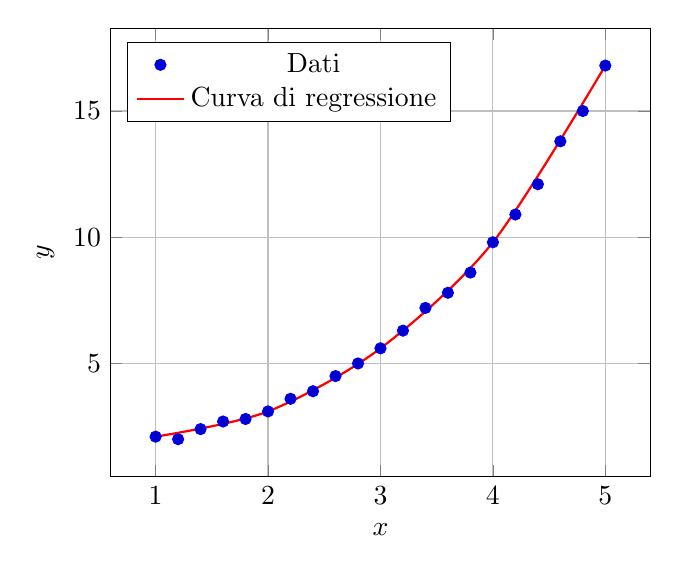
\begin{tikzpicture}
    \begin{axis}[
        xlabel=$x$,
        ylabel=$y$,
        legend pos=north west,
        grid=major
    ]

    % 1. Dati originali (solo punti)
    \addplot+[only marks, mark=*, mark size=2pt] 
        table[row sep=\\] {
        x  y \\
        1.0 2.1 \\
        1.2 2.0 \\
        1.4 2.4 \\
        1.6 2.7 \\
        1.8 2.8 \\
        2.0 3.1 \\
        2.2 3.6 \\
        2.4 3.9 \\
        2.6 4.5 \\
        2.8 5.0 \\
        3.0 5.6 \\
        3.2 6.3 \\
        3.4 7.2 \\
        3.6 7.8 \\
        3.8 8.6 \\
        4.0 9.8 \\
        4.2 10.9 \\
        4.4 12.1 \\
        4.6 13.8 \\
        4.8 15.0 \\
        5.0 16.8 \\
        };

    % 2. Retta di regressione (calcolata automaticamente sui dati)
    \addplot+[
    smooth,
    no markers, 
    thick, 
    red
    ] 
    table[
        row sep=\\
        %y={create col/linear regression={y=y}}
    ]{
        x  y \\
        1  2.1 \\
        2  3.1 \\
        3  5.6 \\
        4  9.8 \\
        5  16.8 \\
        };

    \legend{Dati, Curva di regressione}
    \end{axis}
\end{tikzpicture}
\end{minipage}

\caption{A sinistra una Regressione Lineare Univariata (Retta). A destra una approssimazione NON Lineare (Curva lisciata)}
\end{figure}
Per chiarezza, la curva di regressione \ref{fig:grafico regressione} è stata creata interpolando solo 5 punti dall'insieme del dataset presi a intervalli regolari. Questo non altera la tendenza poiché la funzione tende a generalizzare bene l'andamento dei punti.\\
Dati un insieme di $i$ punti con 2 variabili $(x,y)$,  per esempio
$(x=\text{Larghezza},y=\text{Lunghezza})$ la regressione è costruire una funzione che adatta l'andamento
dei punti. In questa tesi si affronterà la Regressione Lineare Univariata. Nella Regressione Lineare Univariata la funzione che adatta i punti è una retta.
La retta viene definita tramite la formula del tipo
\[
y=mx+q
\] 
Ove $m$ indica l'inclinazione della retta, mentre $q$ è lo spostamento di quella retta sull'asse delle ordinate.
Si vuole trovare la funzione $f$ che approssimi la sequenza dei vari punti.
Quindi date $i$ coppie $(x_i,y_i)$ questo problema si risolve utilizzando il Metodo Dei Minimi Quadrati. 
\begin{align}
    m&=\frac{i\cdot \sum x_iy_i- \sum x_i \cdot \sum y_i}
    {i \cdot \sum (x_i^2)- \left(\sum x_i \right)^2}\\
    q&=\frac{\sum y_i \cdot \sum (x_i^2)- \sum x_i \cdot \sum x_iy_i}
    {i \cdot \sum (x_i^2)- \left(\sum x_i \right)^2}
\end{align}

Di conseguenza si può costruire la precedente funzione $f$ che dà il punto sull'ordinata $y_i$ sapendo solo il punto sulle ascisse $x_i$.
\[
f(x_i)=m\cdot x_i+q=y_i
\]

Ulteriori approfondimenti sul Machine Learning si possono affrontare nel libro \cite{russell2010artificial} o nella sua versione in italiano \cite{Russell2022-re}

\subsection{Normalizzazione e filtratura di un dataset}
\label{subsec:normalizzazione_dataset}
Per normalizzazione di un dataset si intende dare a un insieme di dati un range garantito. 
Per farlo si usa la seguente formula: dato un insieme di dati $X$ di numero $i$, 
\[
    x_i=\frac{x_i-\min(X)}{\max(X)-\min(X)}
\]
Dove $X$ è il vettore che contiene tutti gli $x_i$. Quindi
\[
    X=\{x_1,x_2,...,x_i\}
\]
In questa tesi si utilizzeranno dei filtri. Nello specifico filtri di media locale e varianza locale tra i vari pixel. 
Si mostra una rappresentazione dei vari pixel \ref{fig:pixel}. 
Supponiamo che $X$ sia il vettore che contiene i valori 
dei pixel rosso.

\begin{figure}[H]
        \centering
        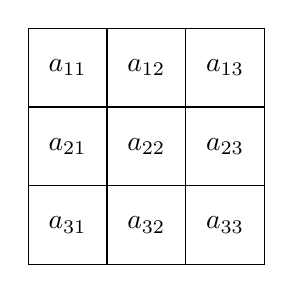
\begin{tikzpicture}[scale=1]

            % Griglia 3x3
            \draw (0,0) rectangle (3,3);
            \draw (1,0) -- (1,3);
            \draw (2,0) -- (2,3);
            \draw (0,1) -- (3,1);
            \draw (0,2) -- (3,2);

            % Etichette
            \node at (0.5,2.5) {$a_{11}$};
            \node at (1.5,2.5) {$a_{12}$};
            \node at (2.5,2.5) {$a_{13}$};

            \node at (0.5,1.5) {$a_{21}$};
            \node at (1.5,1.5) {$a_{22}$};
            \node at (2.5,1.5) {$a_{23}$};

            \node at (0.5,0.5) {$a_{31}$};
            \node at (1.5,0.5) {$a_{32}$};
            \node at (2.5,0.5) {$a_{33}$};

        \end{tikzpicture}
        \caption{Esempio pixel}
        \label{fig:pixel}
\end{figure}
Si pone per esempio la seguente griglia ($3x3$) di visualizzazione 
dei valori dei pixel di colore rosso e si pongono i seguenti valori:
\begin{align}
    a_{11}=0.75;a_{12}=0.75;a_{13}=0.75;\\
    a_{21}=0.45;a_{22}=0.25;a_{23}=0.95;\\
    a_{31}=0.35;a_{32}=0.25;a_{33}=0.05;
\end{align}

Di conseguenza nel pixel $a_{22}$ si avrà la media effettuata da:
\begin{align}
    \mathrm{media}_{3\times3,\mathrm{rosso}}(a_{22})&=\frac{1}{i\cdot j}\cdot\sum_i\sum_j a_{ij}\\
    &=\frac{1}{3\cdot3}\cdot \big( \left( 0.75+0.75+0.75\right)\\
    &+ \left( 0.45+0.25+0.95\right)+ \left(0.35+0.25+0.05\right)\big)\\
    &=0.5056
\end{align} 

Quindi nel layer media3x3rosso avremmo nel pixel $a_{22}=0.5056$. 
Nel caso si voglia calcolare la media3x3rosso nel pixel $a_{11}$. Per gestire i pixel nei bordi si specchiano i valori nei pixel. Si creano delle caselle virtuali $a_{00},a_{01},a_{10},...$ all'interno delle quali 
verrà inserito il valore del pixel rosso adiacente. Quindi $a_{00}=a_{01}=a_{10}=a_{11}=0.75$, per $a_{02}=a_{12}=0.75$, per $a_{20}=a_{21}=0.45$ e così via...
Di conseguenza la media nel pixel $a_{11}$ sarà
\begin{align}
    \mathrm{media}_{3\times3,\mathrm{rosso}}(a_{11})&=\frac{1}{i\cdot j}\cdot\sum_i\sum_j a_{ij}\\
    &=\frac{1}{3\cdot3}\cdot \big( \left( 0.75+0.75+0.75\right)\text{ che sarebbe ($a_{00},a_{01},a_{02}$)}\\
    &+ \left( 0.75+0.75+0.75\right) + \left( 0.45+0.45+0.25\right)\big)\\
    &=0.6278
\end{align}
Nella figura la tecnica di fare una media3x3 o 7x7 si rappresenta con una sfocatura \ref{fig:immagine mean3x3}. Si mostrano degli esempi.
%qua ci metti un immagine che mostra la sfocatura

\begin{figure}[H]
    \centering
    \begin{minipage}{0.30\textwidth}
    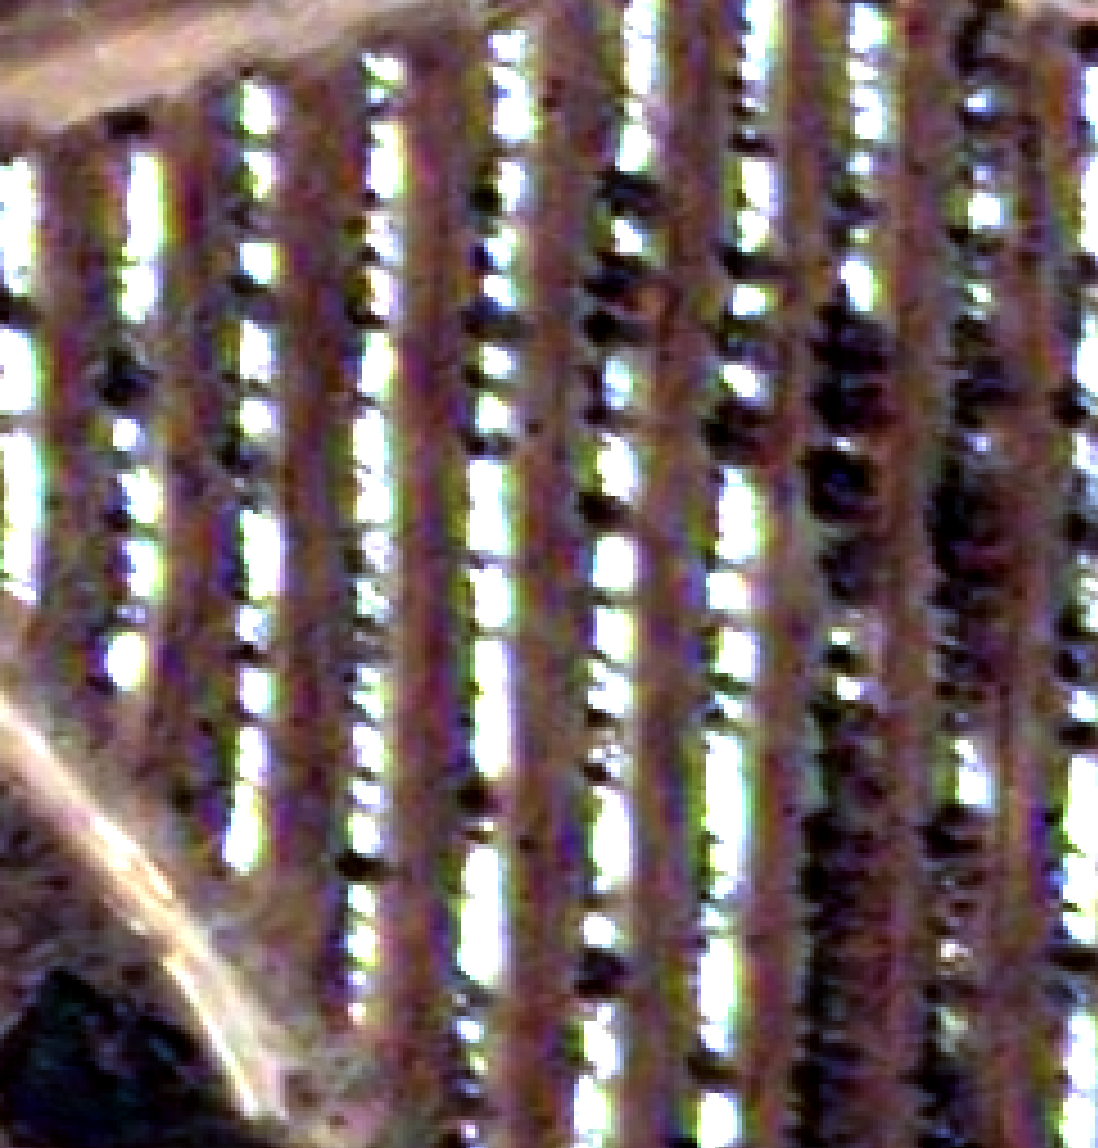
\includegraphics[width=0.7\textwidth]{capitoli/capitolo1/images/rgb.png}
    \caption{Rappresentazione della immagine rosso, verde, blu}
    \label{fig:immagine rgb}
    \end{minipage}
    \hfil 
    \begin{minipage}{0.30\textwidth}
    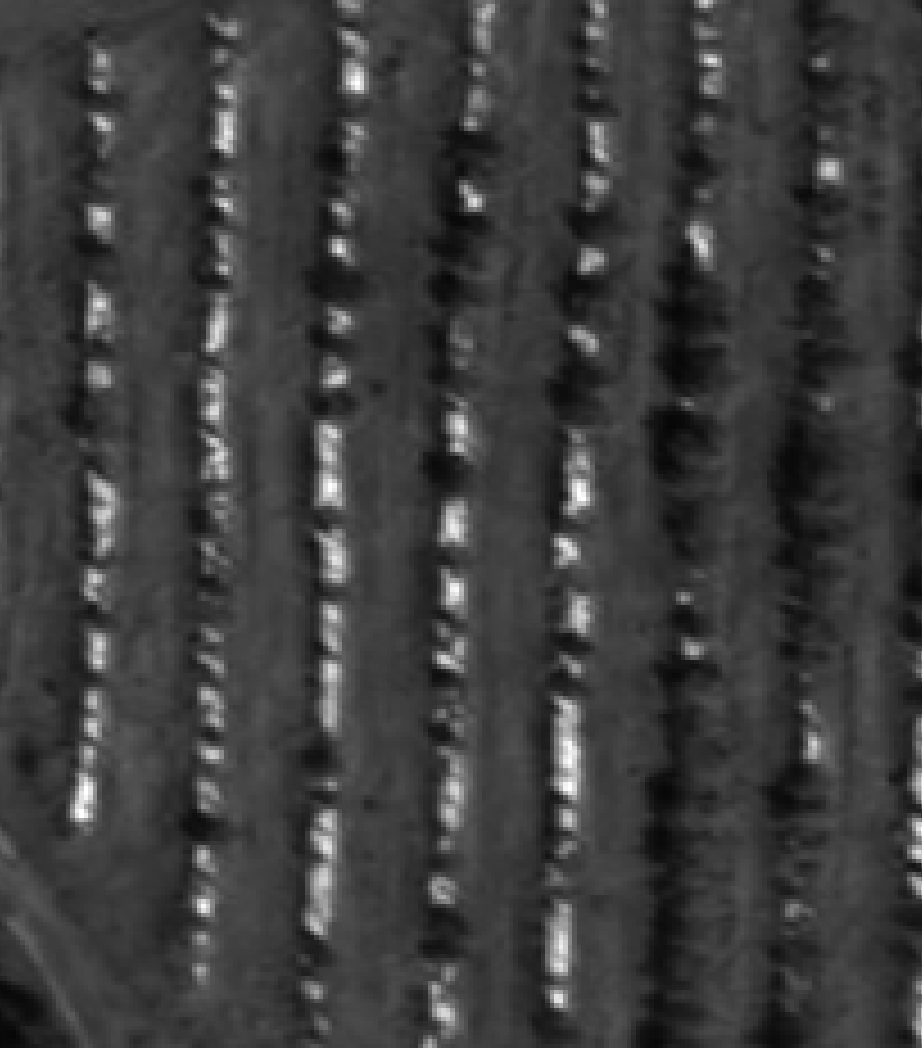
\includegraphics[width=0.7\textwidth]{capitoli/capitolo1/images/RED.png}
    \caption{Rappresentazione della deviazione standard del colore rosso in modo binario (bianco/nero)}
    \label{fig:immagine red}
    \end{minipage}
    \hfil
    \begin{minipage}{0.30\textwidth}
    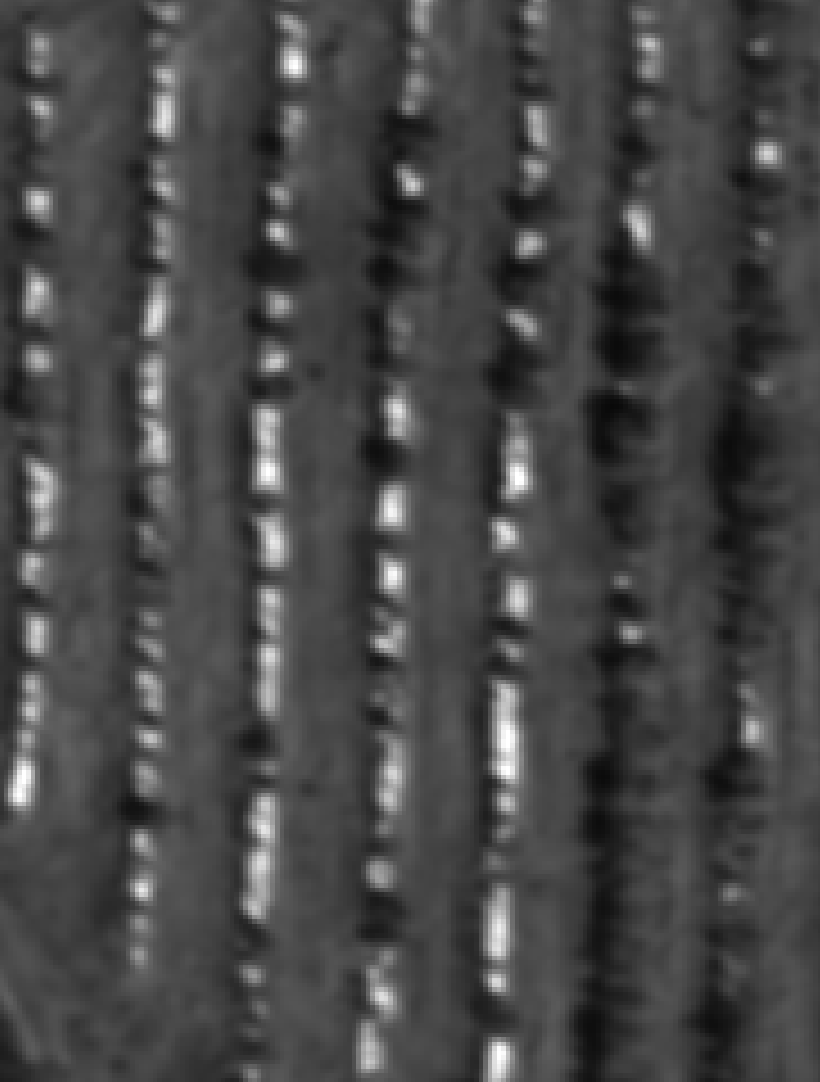
\includegraphics[width=0.7\textwidth]{capitoli/capitolo1/images/mean3x3.png}
    \caption{Rappresentazione della media3x3 del colore rosso in modo binario (bianco/nero)}
    \label{fig:immagine mean3x3}
    \end{minipage}
\end{figure}



La deviazione standard per il pixel $a_{22}$ (in questo caso di colore rosso) è data dalla formula
%\begin{align}
    %devstand3x3rosso(a_{22})&=\sqrt{\frac{1}{i\cdot j} \sum_{i}\sum_{j}  \left( x_{ij}-media3x3rosso(a_{22}) \right)^2}\\
    %&=\sqrt{\frac{1}{3\cdot 3} \big(\left((0.75-0.5056)^2+(0.75-0.5056)^2+(0.75-0.5056)^2\right)\\
    %&+\left((0.45-0.5056)^2+(0.25-0.5056)^2+(0.95-0.5056)^2\right)\\
    %&+ \left((0.35-0.5056)^2+(0.25-0.5056)^2+(0.05-0.5056)^2\right)}}\big)\\
    %&= \sqrt{0.0824}=0.2871
%\end{align}
\begin{align}
\mathrm{devstand}_{3\times3,\mathrm{rosso}}(a_{22})
&=\sqrt{\frac{1}{i\cdot j} \sum_{i}\sum_{j}  \left( x_{ij}-\mathrm{media}_{3\times3,\mathrm{rosso}}(a_{22}) \right)^2}\\
&=
\sqrt{
    \frac{1}{3\cdot3}
    \begin{aligned}[t]
    \Big(
        &(0.75-0.5056)^2+(0.75-0.5056)^2+(0.75-0.5056)^2 \\
        &+(0.45-0.5056)^2+(0.25-0.5056)^2+(0.95-0.5056)^2 \\
        &+(0.35-0.5056)^2+(0.25-0.5056)^2+(0.05-0.5056)^2
    \Big)
    \end{aligned}
} \\
&= \sqrt{0.0824} \approx 0.2872
\end{align}
Anche in questo caso nel caso si voglia calcolare 
$a_{11}$ i valori vengono specchiati come 
nel caso precedente, quindi
\begin{align}
\mathrm{devstand}_{3\times3,\mathrm{rosso}}(a_{11})
&=\sqrt{\frac{1}{i\cdot j} \sum_{i}\sum_{j}  \left( x_{ij}-\mathrm{media}_{3\times3,\mathrm{rosso}}(a_{11})) \right)^2}\\
&=
\sqrt{
    \frac{1}{3\cdot3}
    \begin{aligned}[t]
    \Big(
        &(0.75-0.6278)^2+(0.75-0.6278)^2+(0.75-0.6278)^2 \\
        &+(0.75-0.6278)^2+(0.75-0.6278)^2+(0.75-0.6278)^2 \\
        &+(0.45-0.6278)^2+(0.45-0.6278)^2+(0.25-0.6278)^2 \Big)
    \end{aligned}
} \\
&= \sqrt{0.0328} \approx 0.1812
\end{align}
La rappresentazione visuale della deviazione standard sul rosso su un'immagine si rappresenta come un 
accentuamento del cambio di intensità del colore \ref{fig:immagine std}. Si visualizza un immagine per esempio.
%qua ci si mette la figura std

    
\begin{figure}[H]
    \centering
    \begin{minipage}{0.45\textwidth}
    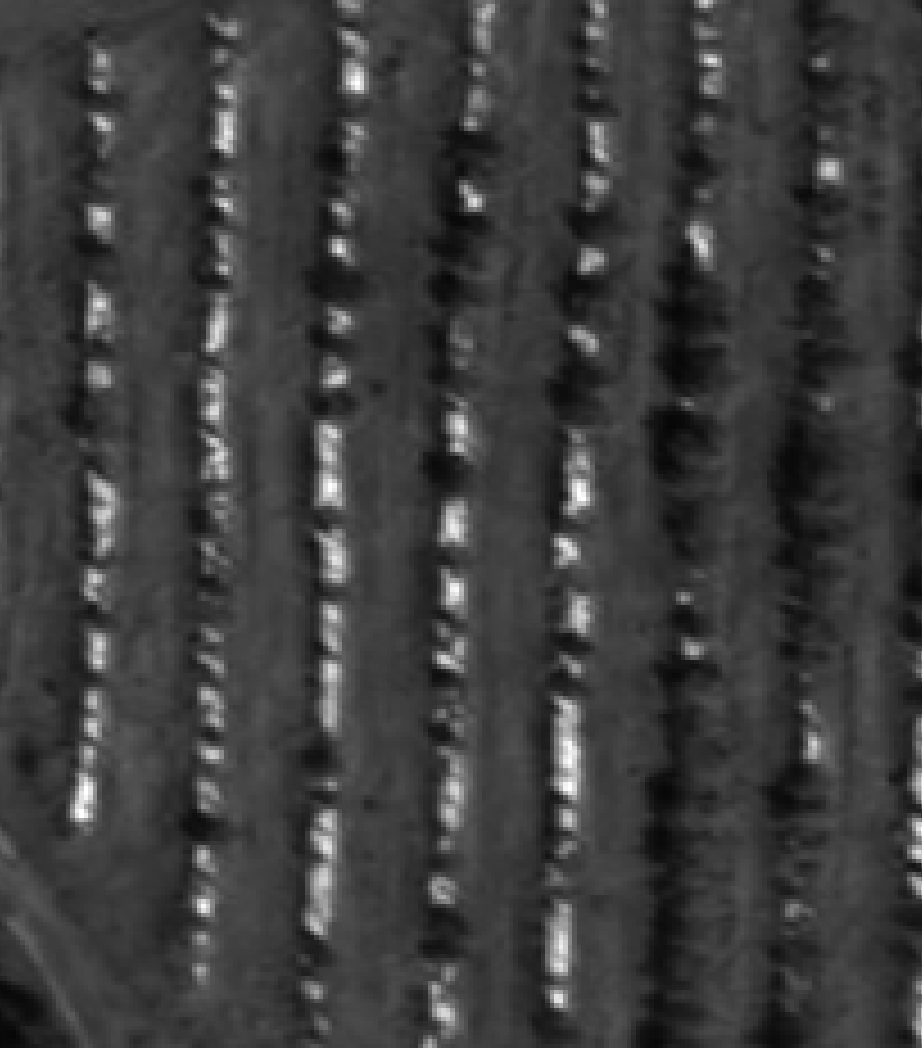
\includegraphics[width=0.7\textwidth]{capitoli/capitolo1/images/RED.png}
    \caption{Rappresentazione del colore rosso in modo binario (bianco/nero)}
    \label{fig:immagine red2}
    \end{minipage}
    \hfil \hfil \hfil
    \begin{minipage}{0.45\textwidth}
    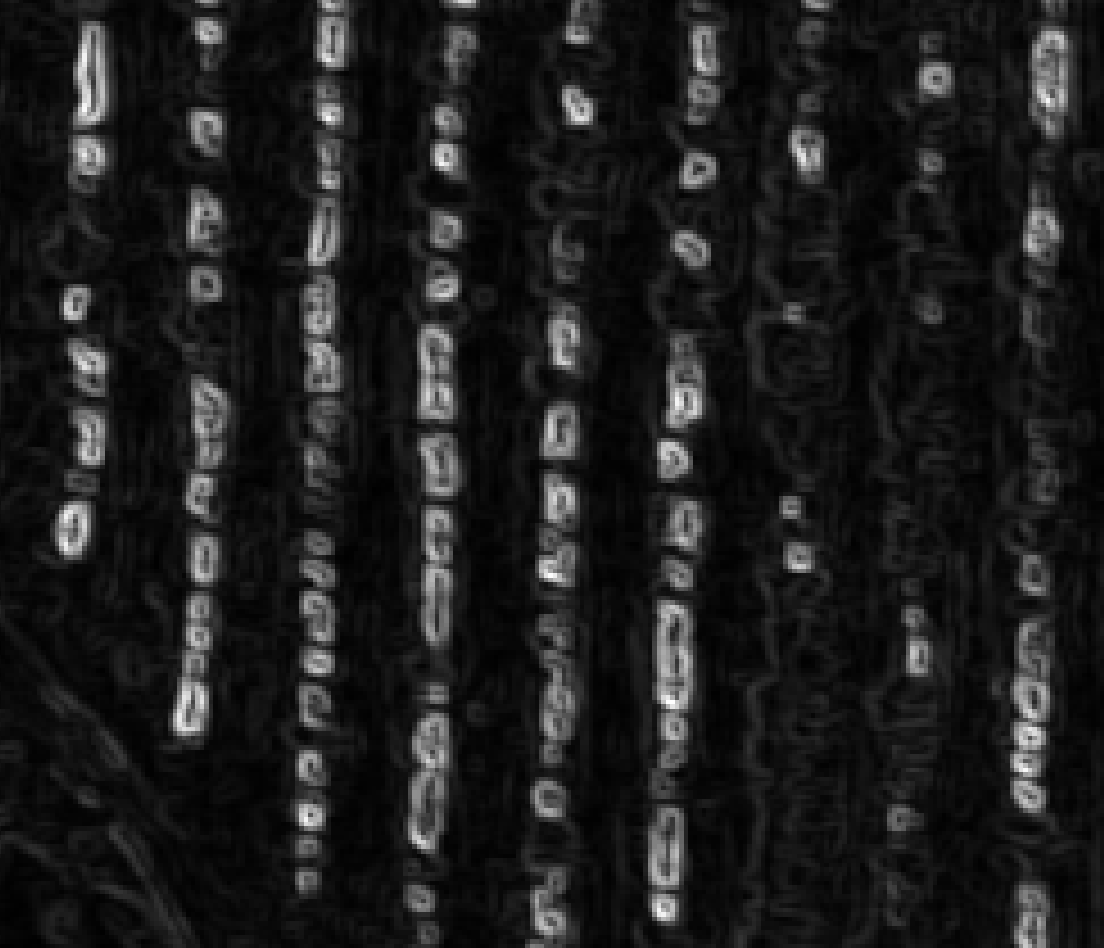
\includegraphics[width=0.7\textwidth]{capitoli/capitolo1/images/std.png}
    \caption{Rappresentazione della deviazione standard del colore rosso in modo binario (bianco/nero)}
    \label{fig:immagine std}
    \end{minipage}
\end{figure}

\section{Metodi noti per la risoluzione del problema}
Il problema di identificare le potenziali piante data un'immagine (in questo caso satellitare) non è banale.
Non si può dedurre che si riuscirà a identificare la pianta in maniera certa e di conseguenza è necessario 
procedere a valutare caso per caso se l'identificazione è possibile.\\
Alcuni articoli, come \cite{YAO2021107591}, hanno usato una rete neurale (di tipologia CNN) per trovare una mappa di densità degli alberi dall'immagine. Il numero totale degli alberi si ottiene integrando tale mappa.
Altri articoli, come \cite{FU2017106}, usano una Foresta Casuale \ref{subsec:foresta_casuale} pixel per pixel per mappare la vegetazione delle zone umide. 
È stata inoltre consultata la tesi \cite{pampalone_tane_fossori} per avere un contesto sulla lavorazione pixel per pixel.

%Stop crea un altro file del capitolo 2
